\chapter{Geant4 Simulations}

In order to provide a new interactive approach to CosmicWatches for new users a scintillation simulation has been devised using the Geant4 toolkit. With this, we intend to showcase some of the physical aspects that may be studied with the detector. This project is still in development and can be found on the GitHub repository \href{https://github.com/spenceraxani/CosmicWatch_Geant4}{CosmicWatch\_Geant4}. This section aims to give a brief explanation of the inner workings of the simulation as well as the Geant4 toolkit.

\section{What is Geant4?}

As defined by the authors \cite{Geant4}, Geant4 is a simulation toolkit based in \texttt{C++}, to model the passage of particles through matter, allowing the creation of custom detector geometries, tracking, and hit recollection, it includes multiple physics models for processes covering a wide range of specialties, such as electromagnetic, hadronic, and optical processes. Its main areas of application are high energy, nuclear, and accelerator physics, as well as medical and space science.

A comprehensive \href{https://geant4-userdoc.web.cern.ch/UsersGuides/InstallationGuide/html/}{installation guide} has been made by the authors, the toolkit is available on Windows, MacOS, and Linux. We recommend building and installing it from source using CMake, since it provides great control over the specific configurations available during installation. Some great tutorials can also be found online, the simulations shown here are based on the architecture illustrated by Physics Matters in his YouTube series \href{https://youtube.com/playlist?list=PLLybgCU6QCGWgzNYOV0SKen9vqg4KXeVL&si=mdzOyTZS0DYsf_vc}{Geant4 Tutorials}.

\section{Geometry}

As noted before, Geant4 allows the creation of custom geometries, which in our use case is great, since it provides a platform suitable for testing multiple CosmicWatch configurations as shown in Sections \labelcref{sec:collected_produced,sec:SiPM_placement,sec:Scint_size,sec:cos_squared}.

In general, Geant4 requires a mother volume in which the simulation will take place, in this case, we have chosen a $20\times20\times20$ \unit{\cm\cubed} box of \texttt{G4\_AIR}\footnote{This and all other materials used in the simulation, are built from the \textit{Geant4 Material Database}, accessed through the \texttt{G4NistManager} class}. The scintillating material is a $5\times5\times1$ \unit{\cm\cubed} box. The sizes of all these elements can of course be changed (as explored in Section \labelcref{sec:Scint_size}) the settings detailed above are just the default configuration in \texttt{headers/construction.hh}. Fig. \ref{fig:geometry} shows the SiPM and scintillator placement inside the mother volume.

\begin{figure}[H]
  \centering
  \begin{subfigure}[t]{0.48\textwidth}
    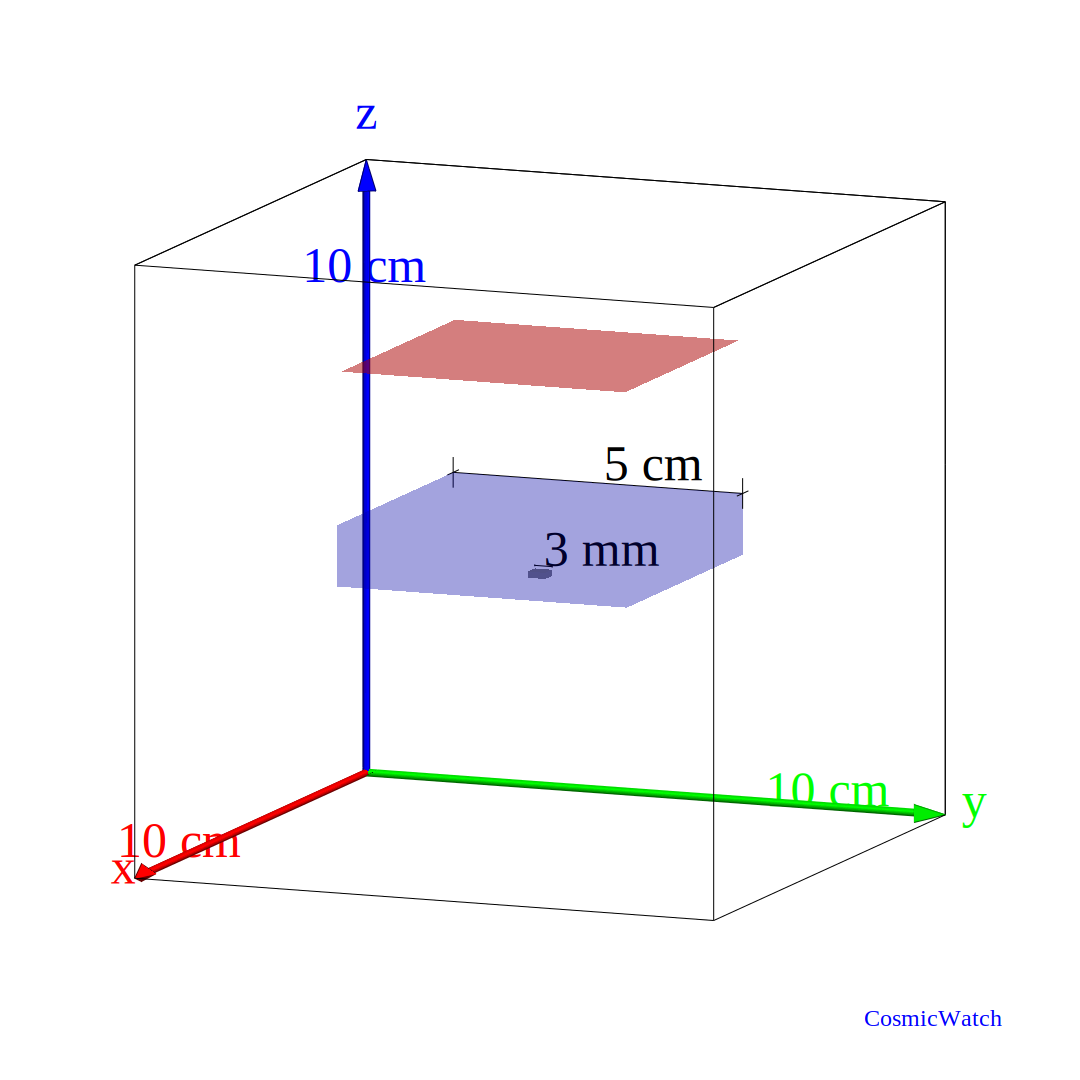
\includegraphics[width=\textwidth]{G4_simulations/profile.pdf}
    \caption{\label{sfig:geometry_profile}Diagonal view.}
  \end{subfigure}
  \hfill
  \begin{subfigure}[t]{0.48\textwidth}
    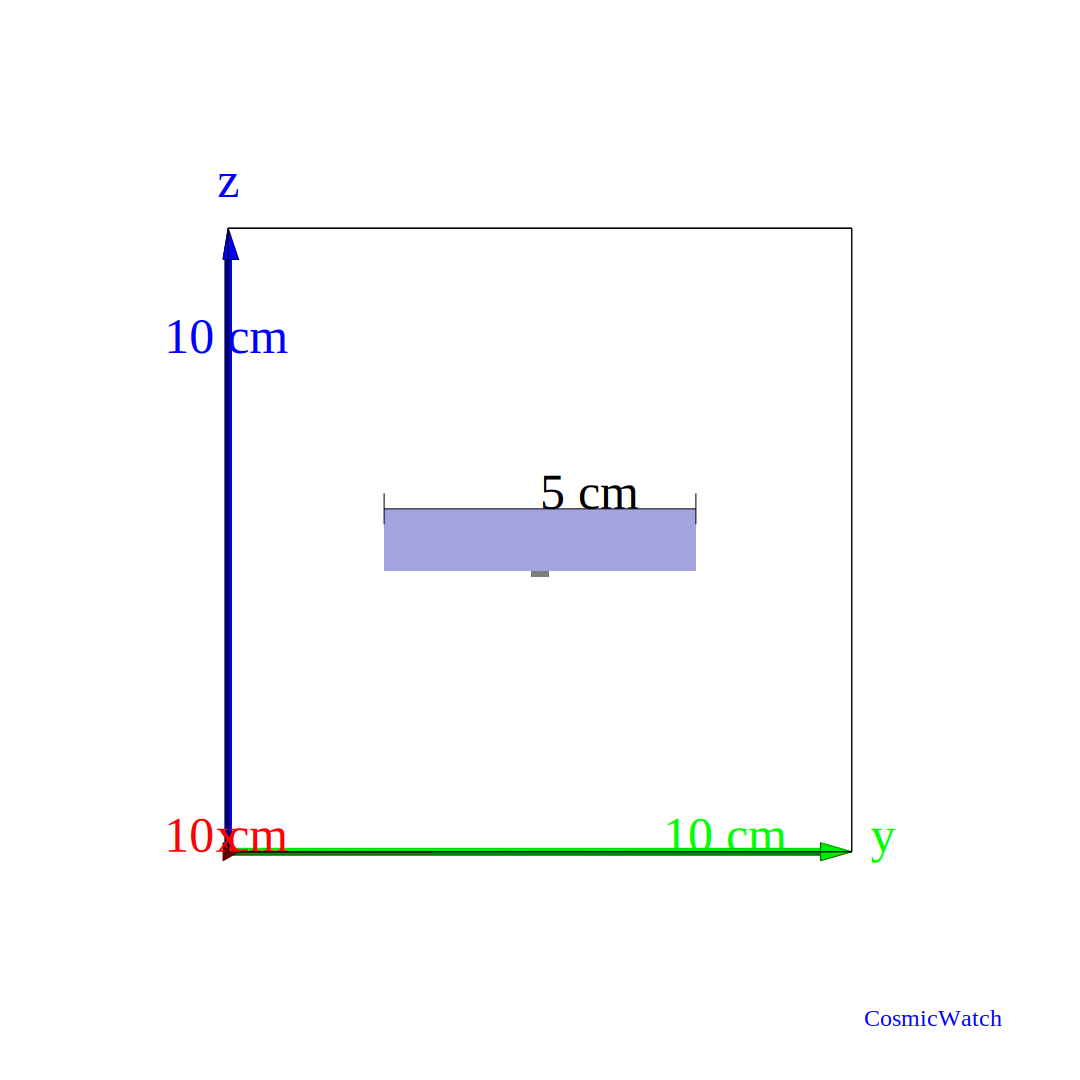
\includegraphics[width=\textwidth]{G4_simulations/front.pdf}
    \caption{\label{sfig:geometry_front}Front view.}
  \end{subfigure}
  \caption{\label{fig:geometry}Scintillator and SiPM placement in the mother volume.}
\end{figure}

For simplicity, the SiPM is also modeled as a box filled with \texttt{G4\_AIR} with dimensions $3\times3\times1$ \unit{\mm\cubed} attached to the base of the scintillator. The detected photons specified in the following subsections are counted as they enter the SiPM volume, this volume-check process is done in \texttt{source/stepAction.cc}, and relevant information for every event is saved to a \texttt{ntuple} by the \texttt{G4GenericAnalysisManager} class as defined in \texttt{source/eventAction.cc}. The simulation speed could be improved by employing the \text{G4VHits} and \texttt{G4THitsCollection} classes, which are optimized to record data for every step inside a sensitive volume in the simulation.

As discussed in \labelcref{sec:self_radiation}, LYSO crystals contain $^{176}$Lu, a naturally occurring radioactive isotope emitting betas. LYSO crystals can absorb their own radiation, resulting in a constant background, this feature however, has not yet been included in the simulation, which is why the scintillating material used is the same as in previous versions of CosmicWatch, a plastic scintillator based on Polyvinyltoluene, the material name in the \textit{Geant4 Material Database} is \texttt{G4\_PLASTIC\_SC\_VINYLTOLUENE}.

\section{Muons going through the scintillator}

The following simulation results were designed to recreate some of the results typically seen with CosmicWatches, they also give insight into some construction characteristics that can be taken into account while building a detector. In order to speed up the simulation, the muons being shot have initial energies of 50 \unit{\mega\eV}, much lower than what would be expected at sea level (4 \unit{\giga\eV}). The particle gun used in this simulation is a \texttt{G4GeneralParticleSource}, the setting of this particle gun can be changed in macro files. Figures TALES show some of the geometries the particle source can have.

\section{Simulation results}

\subsection{Photons collected vs. produced}\label{sec:collected_produced}

\subsection{SiPM placement}\label{sec:SiPM_placement}

The collocation of the SiPM can be a factor to keep in mind while designing new CosmicWatch setups. Generally, the photomultiplier is located on the base of the scintillator as shown in Figure \ref{fig:geometry}, but it may be useful to place it on one of its sides as shown in Fig. \ref{fig:SiPM_side}.

\begin{figure}[H]
  \centering
  \begin{subfigure}[t]{0.48\textwidth}
    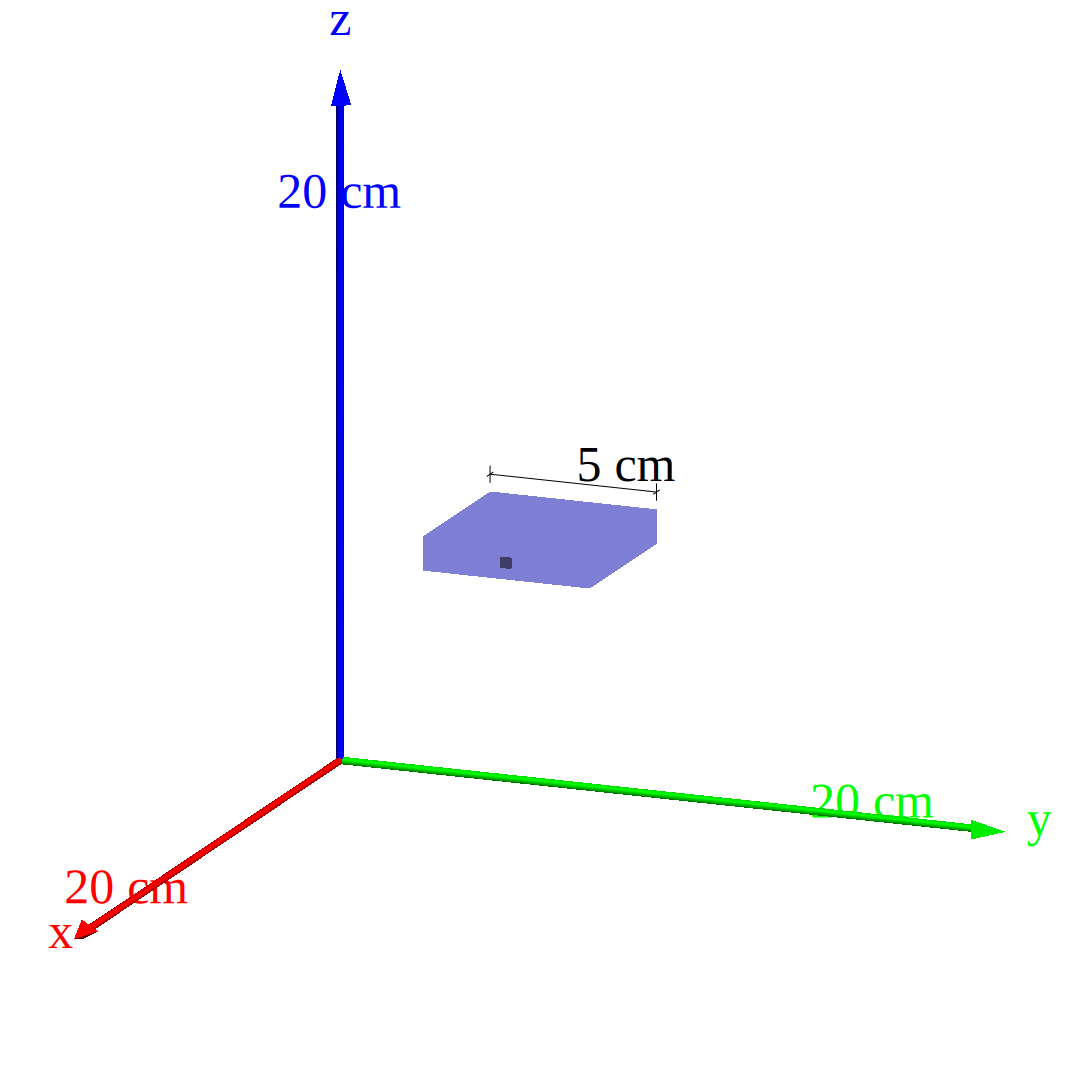
\includegraphics[width=\textwidth]{G4_simulations/SiPM_side_profile.pdf}
    \caption{\label{sfig:SiPM_side_profile}Diagonal view.}
  \end{subfigure}
  \hfill
  \begin{subfigure}[t]{0.48\textwidth}
    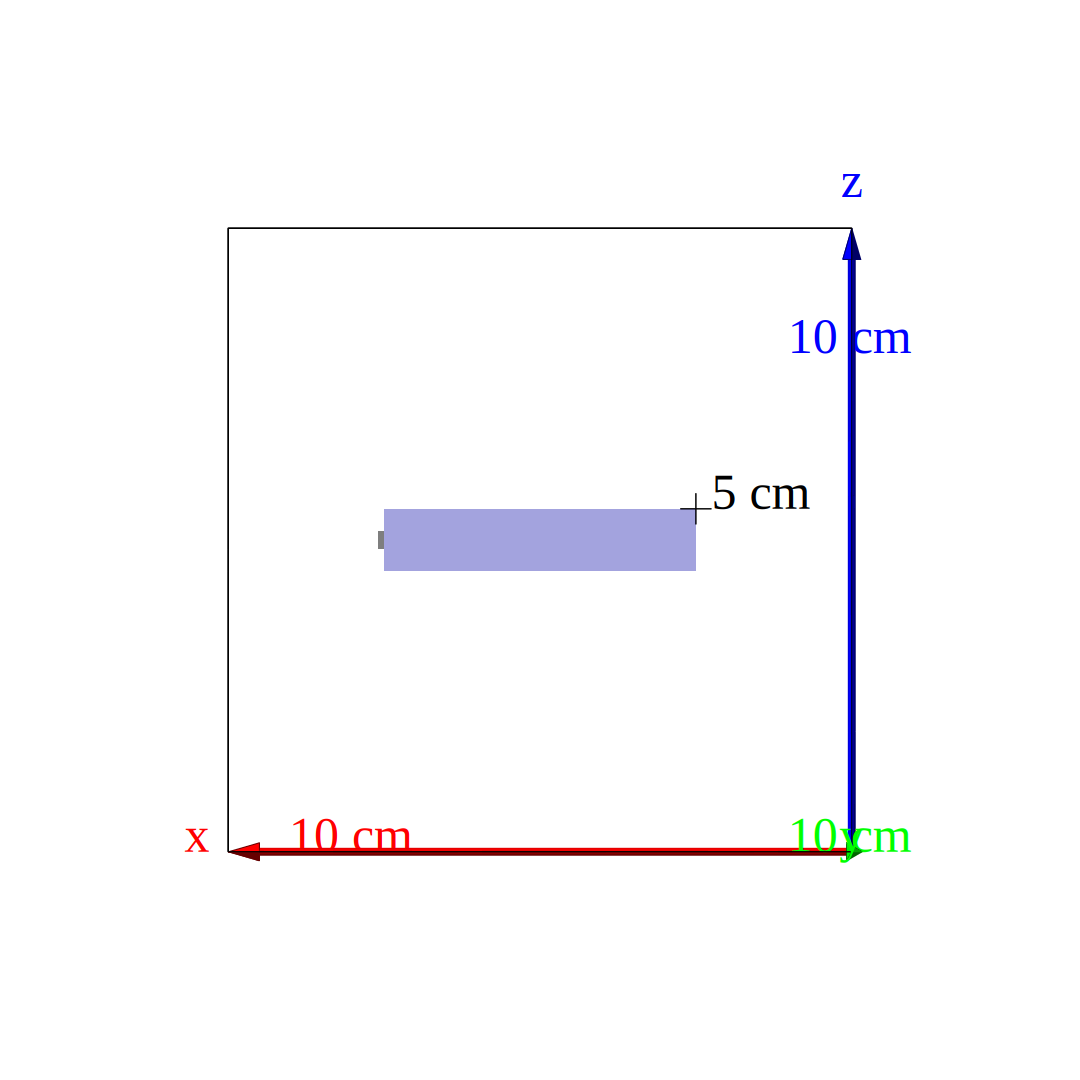
\includegraphics[width=\textwidth]{G4_simulations/SiPM_side_front.pdf}
    \caption{\label{sfig:SiPM_side_front}Side view.}
  \end{subfigure}
  \caption{\label{fig:SiPM_side}SiPM placed on the front face of the scintillator.}
\end{figure}

\begin{figure}[H]
    \centering
    \begin{subfigure}[t]{0.48\textwidth}
      \includegraphics[width=\textwidth]{G4_simulations/run0_nt_Event_SiPM-placement_energy_spectra.pdf}
      \caption{\label{sfig:SiPM_place_edep}Energy deposition in the detector for different photomultiplier placements.}
    \end{subfigure}
    \hfill
    \begin{subfigure}[t]{0.48\textwidth}
      \includegraphics[width=\textwidth]{G4_simulations/run0_nt_Event_SiPM-placement_photon_count.pdf}
      \caption{\label{sfig:SiPM_place_pcount}SiPM photon count for both setups.}
    \end{subfigure}
    \caption{\label{fig:SiPM_place_results}Wenas.}
\end{figure}

As expected, the energy deposition in the crystal should not depend on the SiPM placement. Surprisingly enough, however, it seems that the photon count is also not affected by this, meaning that the results obtained with both setups should be similar while using the specified scintillator size.

\subsection{Scintillator sizes}\label{sec:Scint_size}

The current architecture of CosmicWatch allows to use of variable scintillator sizes, the first versions of CosmicWatch used 5$\times$5$\times$1 \unit{\cm\cubed} scintillators, while the newer LYSO crystals are much smaller, Fig. \ref{fig:LYSO_crystals} shows some of the crystals used while testing the detector response. This simulation aims at understanding the effects of variable sizes in the final results.

\begin{figure}
  \centering
    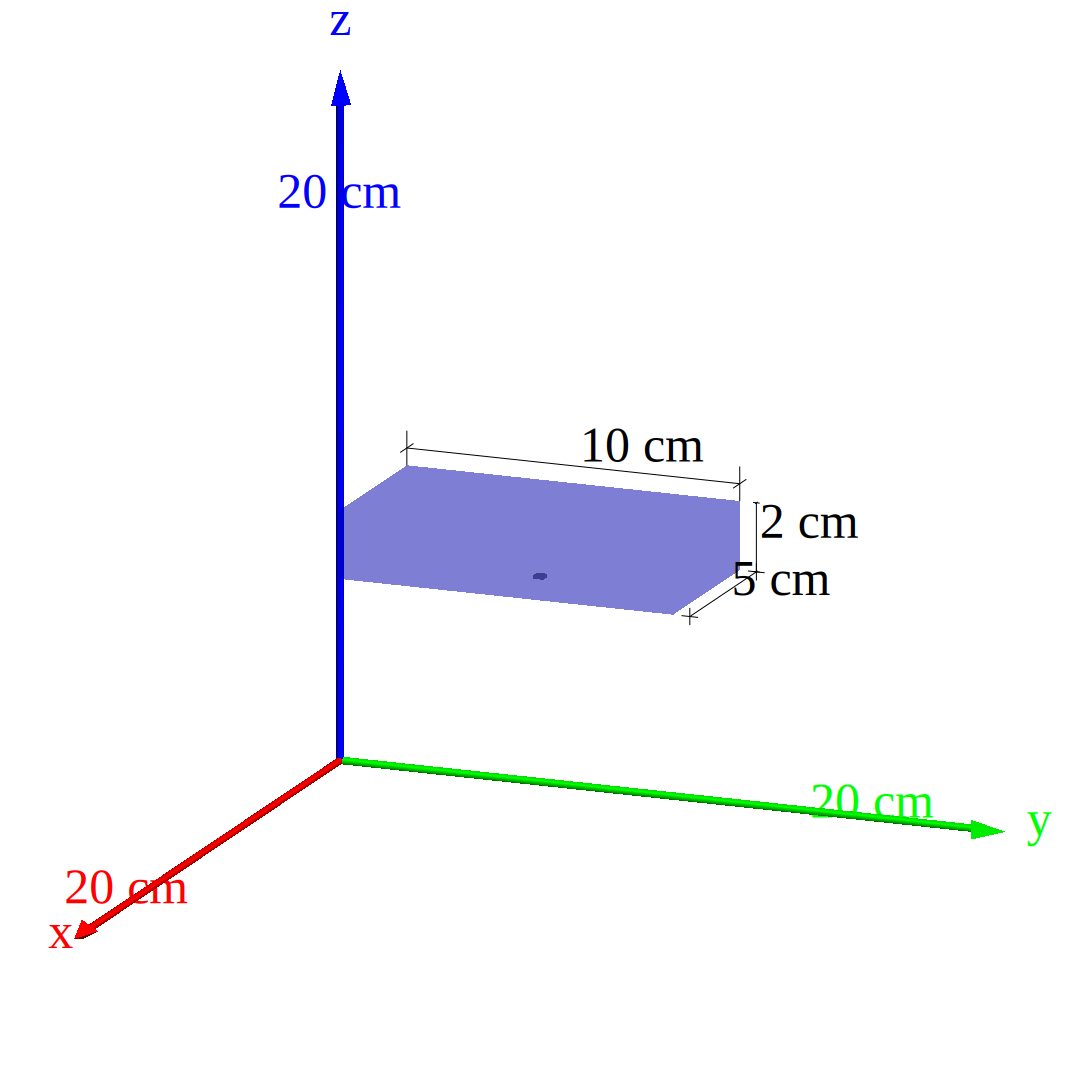
\includegraphics[width=0.47\textwidth]{G4_simulations/Scint_size_10_5_2.pdf}
  \caption{\label{fig:Scint_10_5_2}Visualization of a bigger scintillator in the mother volume.}
\end{figure}

\begin{figure}
  \centering
  \begin{subfigure}[t]{0.48\textwidth}
    \includegraphics[width=\textwidth]{G4_simulations/run0_nt_Event_crystal-size_energy_spectra.pdf}
    \caption{\label{sfig:scint_size_edep}Energy deposition in the detector for different scintillator sizes.}
  \end{subfigure}
  \hfill
  \begin{subfigure}[t]{0.48\textwidth}
    \includegraphics[width=\textwidth]{G4_simulations/run0_nt_Event_crystal-size_photon_count.pdf}
    \caption{\label{sfig:scint_size_pcount}SiPM photon count for different scintillator sizes.}
  \end{subfigure}
  \caption{\label{fig:scint_size_results}The scintillator size can be easily chosen inside the simulation by changing the values of \texttt{PScintXLen}, \texttt{PScintYLen}, and \texttt{PScintZLen} in \texttt{headers/construction.hh}.}
\end{figure}

Figure \ref{sfig:scint_size_edep} shows that bigger SiPM sizes do result in greater energy recollections, however, as Figure \ref{sfig:scint_size_pcount} illustrates, the number of photons that reached the SiPM was on average greater for the $5\times5\times1$ \unit{\cm\cubed} setup. These figures then show that increased scintillator volume does not directly correlate with photon counts in the SiPM, which is ultimately the goal of the detector, to collect as many photons as possible in the photomultiplier to increase energy resolution.

\subsection{Angular distributions}\label{sec:cos_squared}

With this simulation, we are trying to understand the detector response as a function of the zenith angle $\theta$, studying the energy deposition in the scintillating material and photon count in the SiPM depending on the trajectory of the particle once it enters the detector. As shown in Figure TALES, a spherical particle source was used to shoot particles from all directions toward the center of the scintillating crystal. This however, does not recreate the cosine squared law, as the particle source is ``isotropic,'' meaning that it does not have a preferred direction to shoot particles from.

\begin{figure}[H]
  \centering
  \begin{subfigure}[t]{0.48\textwidth}
    \includegraphics[width=\textwidth]{G4_simulations/run0-ang_dis_nt_Event_energy_spectra.pdf}
    \caption{\label{sfig:ang_edep}Energy deposition in the detector as a function of zenith angle.}
  \end{subfigure}
  \hfill
  \begin{subfigure}[t]{0.48\textwidth}
    \includegraphics[width=\textwidth]{G4_simulations/run0-ang_dis_nt_Event_photon_count.pdf}
    \caption{\label{sfig:ang_pcount}SiPM photon as a function of zenith angle.}
  \end{subfigure}
  \medskip
  \begin{subfigure}[t]{0.48\textwidth}
    \includegraphics[width=\textwidth]{G4_simulations/test_nt_Event_energy_spectra.pdf}
    \caption{\label{sfig:ang_edep_cylinder}Energy deposition in the detector as a function of zenith angle with a cylindrical scintillator.}
  \end{subfigure}
  \hfill
  \begin{subfigure}[t]{0.48\textwidth}
    \includegraphics[width=\textwidth]{G4_simulations/test_nt_Event_photon_count.pdf}
    \caption{\label{sfig:ang_pcount_cylinder}SiPM photon as a function of zenith angle with a cylindrical scintillator.}
  \end{subfigure}
  \caption{\label{fig:ang_results}Data in blue is the raw output of the simulation while shooting muons directly toward the center of the scintillator. Data in orange is the normalization of the simulation output using a cosine squared law.}
\end{figure}

As can be seen in Figure TALES, muons traveling directly downward have less scintillating material to go through compared to those traveling horizontally, this means that greater zenith angles should result in greater energy depositions, which agrees with the data shown in Figures \ref{sfig:ang_edep} and \subref{sfig:ang_edep_cylinder}. In Figure \ref{sfig:ang_pcount} however, the photon count first decreases to a minimum at around 30$^\circ$ to then steadily increase until 90$^\circ$. Based on what we learned in the previous section \ref{sec:Scint_size} about scintillator sizes, and keeping in mind the detector geometry, one would expect a minimum photon count at the angle where the photons have to travel the greatest distance, which in this case corresponds the scintillator edges an corners, ranging between 78.69 and 81.95 degrees for a $5\times5\times1$ \unit{\cm\cubed} scintillator.

In order to attenuate any possible polar dependencies, the scintillator geometry was changed to a cylinder as shown in Figure TALES. This however, does not seem to correlate with the presence of a minimum in photon count at 30$^\circ$, as can be seen in Figure \ref{sfig:ang_pcount_cylinder}.

\subsection{Simulated Spectra}

Contrary to \texttt{G4\_PLASTIC\_SC\_VINYLTOLUENE} and \texttt{G4\_Air}, there is no \texttt{G4\_LYSO}, which in this case is needed to produce gamma-spectra since this plastic scintillator does not produce enough photoelectric events to obtain something similar to the spectra shown in Section \ref{sec:gammas_in_the_detector}. Luckily Geant4 allows to create materials by adding individual elements with their respective percentage in the compound. Table \ref{tab:LYSO_composition} shows the specific percentages for all elements that make up a LYSO. In order to add Cerium doping one can create a new material made of two parts, LYSO and Ce, in this case, one would use the doping percentage to calculate the amount of LYSO in the new compound. It hasn't been possible to find the specific amount of Ce doping in Luxium's LYSO, there are however some publications that reference doping below 1.\% for Saint-Gobain samples \cite{Ce_doping,Ce_dopping_2}\footnote{Luxium and Saint-Gobain's LYSOs are essentially the same since Luxium acquired the scintillation and photonic crystals business of Saint-Gobain.}. All material definitions can be found under the function \texttt{DefineMaterials} of \texttt{MyDetectorConstruction} class in \texttt{source/construction.cc}.

\begin{table}[H]
  \caption{Atomic mass and composition percentage for all elements in the nominal composition Lu$_{1.8}$Y$_{0.2}$SiO$_5$:Ce.}
  \centering
  \begin{tabular}{ c c c c c}
    \midrule
     & Lu & Y & Si & O \\
    \midrule
    atomic mass [amu] & 174.967 & 88.906 & 28.086 & 15.999 \\
    \% & 71.447 & 4.034 & 6.371 & 18.148 \\
    \bottomrule
  \end{tabular}
  \label{tab:LYSO_composition}
\end{table}

Figure \ref{fig:LYSO_size_results} shows the obtained energy spectra and SiPM photon count while shooting a monoenergetic gamma-ray. In Figure \ref{sfig:LYSO_size_edep} we see almost a Dirac delta at 662 \unit{\kilo\eV} since this is the Monte Carlo truth, no noise is introduced while adding the energy deposition. It is interesting, however, to see that the counts drop to zero between the Compton edge at 478 \unit{\kilo\eV} and the photopeak, as one would expect.

In Figure \ref{sfig:LYSO_size_pcount} notably, the photomultiplier seems to collect fewer photons from bigger crystals, this could mean that many of them are being attenuated inside the crystal on their path tho the SiPM.

\begin{figure}
  \centering
  \begin{subfigure}[t]{0.48\textwidth}
    \includegraphics[width=\textwidth]{G4_simulations/LYSO_run0_base_crystal-size_energy_spectra.pdf}
    \caption{\label{sfig:LYSO_size_edep}Energy deposition in a LYSO crystal while shooting a monoenergetic 662 \unit{\kilo\eV} gamma ray.}
  \end{subfigure}
  \hfill
  \begin{subfigure}[t]{0.48\textwidth}
    \includegraphics[width=\textwidth]{G4_simulations/LYSO_run0_base_crystal-size_photon_count.pdf}
    \caption{\label{sfig:LYSO_size_pcount}SiPM photon count while shooting a monoenergetic 662 \unit{\kilo\eV} gamma ray.}
  \end{subfigure}
  \caption{\label{fig:LYSO_size_results}Energy deposition and photon count for various LYSO sizes.}
\end{figure}
